\documentclass{article}
\usepackage[margin=0.2in,paperwidth=9in,paperheight=4.8in]{geometry}
\pagestyle{empty}
\usepackage{amsmath,amssymb}
\usepackage{tikz}
\usetikzlibrary{shapes.geometric, arrows.meta, positioning, calc}

\begin{document}
\noindent
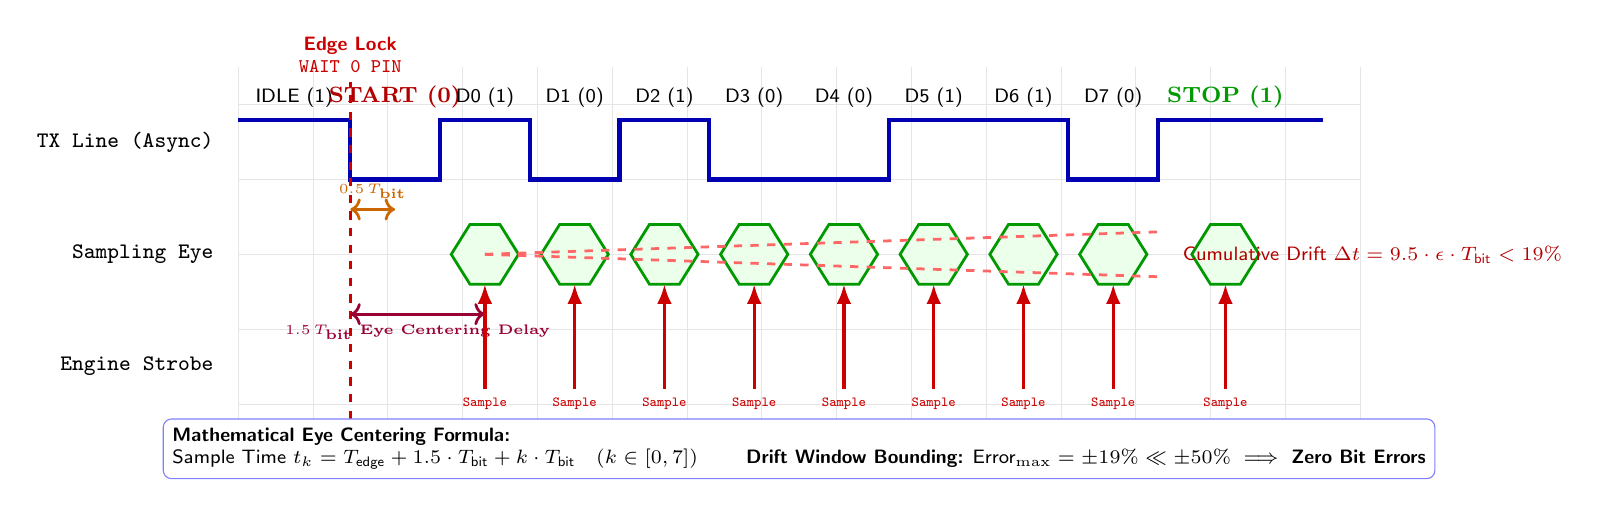
\begin{tikzpicture}[
    scale=0.95,
    wave/.style={line width=1.5pt, blue!70!black},
    strobe/.style={-{Latex[length=2.5mm]}, line width=1.2pt, red!80!black},
    drift/.style={line width=1pt, dashed, gray!60},
    txt/.style={font=\scriptsize\sffamily}
]

% Background grid
\draw[help lines, color=gray!20, ystep=1, xstep=1] (0,-0.5) grid (15,4.5);

% Signal labels
\node[font=\footnotesize\ttfamily, anchor=east] at (-0.2, 3.5) {TX Line (Async)};
\node[font=\footnotesize\ttfamily, anchor=east] at (-0.2, 2.0) {Sampling Eye};
\node[font=\footnotesize\ttfamily, anchor=east] at (-0.2, 0.5) {Engine Strobe};

% UART Waveform: Idle (1) -> Start (0) -> D0 (1) -> D1 (0) -> D2 (1) -> D3 (0) -> D4 (0) -> D5 (1) -> D6 (1) -> D7 (0) -> Stop (1)
\draw[wave] (0, 3.8) -- (1.5, 3.8) -- (1.5, 3.0) -- (2.7, 3.0) % Start bit
            -- (2.7, 3.8) -- (3.9, 3.8) -- (3.9, 3.0) % D0=1, D1=0
            -- (5.1, 3.0) -- (5.1, 3.8) -- (6.3, 3.8) -- (6.3, 3.0) % D2=1
            -- (8.7, 3.0) -- (8.7, 3.8) -- (11.1, 3.8) -- (11.1, 3.0) % D3=0, D4=0, D5=1, D6=1
            -- (12.3, 3.0) -- (12.3, 3.8) -- (14.5, 3.8); % D7=0, Stop=1

% Bit labels
\node[txt] at (0.75, 4.1) {IDLE (1)};
\node[txt, text=red!70!black, font=\footnotesize\bfseries] at (2.1, 4.1) {START (0)};
\node[txt] at (3.3, 4.1) {D0 (1)};
\node[txt] at (4.5, 4.1) {D1 (0)};
\node[txt] at (5.7, 4.1) {D2 (1)};
\node[txt] at (6.9, 4.1) {D3 (0)};
\node[txt] at (8.1, 4.1) {D4 (0)};
\node[txt] at (9.3, 4.1) {D5 (1)};
\node[txt] at (10.5, 4.1) {D6 (1)};
\node[txt] at (11.7, 4.1) {D7 (0)};
\node[txt, text=green!60!black, font=\footnotesize\bfseries] at (13.2, 4.1) {STOP (1)};

% Edge Lock at t=0
\draw[line width=1.2pt, red!80!black, dashed] (1.5, -0.2) -- (1.5, 4.3);
\node[txt, red!80!black, align=center, anchor=south] at (1.5, 4.3) {\textbf{Edge Lock}\\\texttt{WAIT 0 PIN}};

% 0.5 Tbit Center Jump
\draw[<->, line width=1pt, orange!80!black] (1.5, 2.6) -- (2.1, 2.6) node[midway, above, font=\tiny\bfseries] {$0.5\,T_{\text{bit}}$};
\draw[<->, line width=1pt, purple!80!black] (1.5, 1.2) -- (3.3, 1.2) node[midway, below, font=\tiny\bfseries] {$1.5\,T_{\text{bit}}$ Eye Centering Delay};

% Sampling Eye Openings
\foreach \x/\b in {3.3/D0, 4.5/D1, 5.7/D2, 6.9/D3, 8.1/D4, 9.3/D5, 10.5/D6, 11.7/D7, 13.2/STOP} {
    % Eye hexagon
    \draw[line width=1pt, green!60!black, fill=green!8] (\x-0.45, 2.0) -- (\x-0.2, 2.4) -- (\x+0.2, 2.4) -- (\x+0.45, 2.0) -- (\x+0.2, 1.6) -- (\x-0.2, 1.6) -- cycle;
    % Strobe arrow
    \draw[strobe] (\x, 0.2) -- (\x, 1.6);
    \node[txt, font=\tiny\ttfamily, red!80!black] at (\x, 0.0) {Sample};
}

% Clock Drift Envelope Cone
\draw[line width=1pt, dashed, red!60] (3.3, 2.0) -- (12.3, 2.3);
\draw[line width=1pt, dashed, red!60] (3.3, 2.0) -- (12.3, 1.7);
\node[txt, red!70!black, anchor=west] at (12.5, 2.0) {Cumulative Drift $\Delta t = 9.5 \cdot \epsilon \cdot T_{\text{bit}} < 19\%$};

% Mathematical Summary Box
\node[draw=blue!50, fill=white, rounded corners=3pt, font=\scriptsize\sffamily, align=left] at (7.5, -0.6) {
    \textbf{Mathematical Eye Centering Formula:} \\
    $\text{Sample Time } t_k = T_{\text{edge}} + 1.5 \cdot T_{\text{bit}} + k \cdot T_{\text{bit}} \quad (k \in [0,7])$ \qquad \textbf{Drift Window Bounding:} $\text{Error}_{\max} = \pm 19\% \ll \pm 50\% \implies \textbf{Zero Bit Errors}$
};

\end{tikzpicture}
\end{document}
